%	Written by 유재성 (2014. 11. 04)
% 이 양식을 사용하기 위해 알아야할 것

% 1. TeX 컴파일러는 ko.TeX Live가 아니라 MikTeX을 사용해야함

% 2. 한글을 사용하기 위해서 kotex 패키지를 use하는데
% 			Miktex 2.9부터는 kotex에 버그가 있어서 잘 안될 것임.
%			그럴 때는 아래 링크대로 kotex을 따로 살치할 것.
% 			http://doeun.blogspot.kr/2012/08/miktex-29-kotex.html

% 3. 한글 논문을 위한 부분, 영문 논문을 위한 부분이 따로 있으니
%			알아서 필요한 부분만 추려 쓸 것.
%			다만 공통되는 부분은 따로 추릴 필요는 없을 것임.

\documentclass[oneside,b5paper,11pt]{book}
%\documentclass[oneside,11pt]{book}

\usepackage[pdftex]{graphicx}
\usepackage{epstopdf}
\usepackage{amsthm}
\usepackage{amsmath}
%\usepackage{geometry} % Package re-sizing page for b5paper
\usepackage[hangul]{kotex} % Korean support
\usepackage{natbib} % cite style
\usepackage{paralist} % package for inline enumerate, i) ii)...
\usepackage{graphicx} % Allows including images
\usepackage{amssymb} % for math symbols
\usepackage{tablefootnote} % to use table foot note
\usepackage[inline]{enumitem} % to use inline enumerate
\usepackage[left=2cm,right=2cm,top=2cm,bottom=2.5cm,b5paper]{geometry}
%\usepackage[left=1.5cm,right=1.5cm,top=3cm,bottom=3cm]{geometry}

%\graphicspath{ {D:/_PlayGround/Github/2016_thesis/tex/images/} } % image files path
\graphicspath{ {C:/My/Playground/Git/2016_Thesis/tex/images/} }

\pagestyle{plain}




\makeatletter
\renewenvironment{thebibliography}[1]
     {\section*{\refname}%
      \@mkboth{\MakeUppercase\refname}{\MakeUppercase\refname}%
      \begin{enumerate}[label={[\arabic{enumi}]},itemindent=*,leftmargin=4em]
      \@openbib@code
      \sloppy
      \clubpenalty4000
      \@clubpenalty \clubpenalty
      \widowpenalty4000
      \sfcode`\.\@m}
     {\def\@noitemerr
       {\@latex@warning{Empty `thebibliography' environment}}%
      \end{enumerate}}
\makeatother




% MATH  ------------------------------------------------------------------

\newcommand{\spart}[1]{\left(#1\right)}
\newcommand{\ppart}[1]{\left[#1\right]}
\newcommand{\norm}[1]{\left|#1\right|}
\newcommand{\med}{\mathrm{median}}
\newcommand {\bm}[1]{\mbox{\boldmath{$#1$}}}
\newcommand {\bb} {{\bm{\beta}}}
\newcommand {\argmin} {\mathop{\rm{argmin}}}

% Line spacing -----------------------------------------------------------
\newlength{\defbaselineskip}
\setlength{\defbaselineskip}{\baselineskip}
\newcommand{\setlinespacing}[1]%
           {\setlength{\baselineskip}{#1 \defbaselineskip}}
\newcommand{\doublespacing}{\setlength{\baselineskip}%
                           {2.0 \defbaselineskip}}
\newcommand{\singlespacing}{\setlength{\baselineskip}{\defbaselineskip}}

%\setlength{\tclineskip}{1.66\baselineskip}
\linespread{1.6}

% Graphic  -----------------------------------------------------------
\DeclareGraphicsRule{.png}{bmp}{}{}


% Table of Contents

% Theorem Style
% THEOREMS ---------------------------------------------------------------
\theoremstyle{plain}
\newtheorem{thm}{Theorem}
\newtheorem{cor}[thm]{Corollary}
\newtheorem{lem}[thm]{Lemma}
\newtheorem{prop}[thm]{Proposition}
%
\theoremstyle{definition}
\newtheorem{defn}{Definition}[chapter]
%
\theoremstyle{remark}
\newtheorem{rem}{Remark}[chapter]
%
\theoremstyle{definition}
\newtheorem{exam}{Example}[chapter]
%
\numberwithin{equation}{chapter}
%\renewcommand{\theequation}{\thesection.\arabic{equation}}
%\setlength{\textwidth 140mm} \setlength{\textheight 200mm}




\begin{document}
%\iffalse
% Cover

%%%%% Cover 1
 \linespread{1.0}
 \thispagestyle{empty}
 \vspace{37mm}
 \begin{center}
 {\Large 석 사 학 위 논 문}
 \end{center}
 \vspace{30mm}
 \begin{center}
 \LARGE 빅데이터 분석을 위한 \\실시간 로지스틱 회귀모형에 관한 연구\\: 베이지안 접근법을 중심으로
 \end{center}
 \vspace{80mm}
 \begin{center}
 {\Large 고 려 대 학 교 ~ 정 책 대 학 원}
 \end{center}
 \begin{center}
 {\Large 데이터 정보학과}
 \end{center}
 \begin{center}
 {\Large 김 \quad\quad 동 \quad\quad 완}
 \end{center}
  \vspace{7mm}
 \begin{center}
 {\Large 2016년 \quad 6월 \quad 일}
 \end{center}
 \linespread{1.6}





\newpage{}
%%%%% Cover 2
 \linespread{1.0}
 \thispagestyle{empty}
 \vspace{15mm}
 \begin{center}
 {\Large 최 태 련 지도교수 \\ 석사학위논문
}
 \end{center}
 \vspace{20mm}
 \begin{center}
 \LARGE 빅데이터 분석을 위한 \\실시간 로지스틱 회귀모형에 관한 연구\\: 베이지안 접근법을 중심으로
 \end{center}
 \vspace{20mm}
 \begin{center}
 {\Large 이 논문을 통계학 석사학위 논문으로 제출함}
 \end{center}
 \vspace{35mm}
 \begin{center}
 {\Large 2016년 \quad 6월 \quad 일}
 \end{center}
 \vspace{20mm}
 \begin{center}
 {\Large 고려대학교 정책대학원}
 \end{center}
 \begin{center}
  {\Large 데이터 정보학과}
 \end{center}
 \begin{center}
 {\Large 김 \quad\quad 동 \quad\quad 완}
 \end{center}
 \linespread{1.6}





\newpage{}		
%%%%% Cover 3
 \linespread{1.0}
 \thispagestyle{empty}
 \vspace{20mm}
 \begin{center}
 {\LARGE 김동완의 통계학 석사학위논문 \\ 심사를 완료함}
 \end{center}
 \vspace{50mm}
 \begin{center}
{\Large 2016년 \quad 6월 \quad 일}
 \end{center}
 \vspace{85mm}
 \begin{center}
 {\Large  \underline{위원장 \hspace{60mm} (인)} \\ \vspace{7mm}
          \underline{위 \quad 원\hspace{60mm} (인)} \\ \vspace{7mm}
          \underline{위 \quad 원\hspace{60mm} (인)} \\ }
 \end{center}
 \linespread{1.6}





\newpage{}
%%%%% Abstract
    \pagenumbering{roman}
    \typeout{Abstract}

\begin{center}
{\Large 국 문 초 록}
\end{center}
\vspace{1cm} {\small \ \indent
본 논문은 배치 방식에 대비되는 온라인 모형 적합 방법을 샘플 수가 수천만건에 이르고 다수의 범주형 변수, 그리고 범주의 개수가 유동적인 대규모 데이터에 적용하기 위한 모형 적합 방법과 해싱을 이용한 가변수 코딩(Feature Hashing)에 대해 고려해 보고 각 방법의 특성에 대해서 고찰하였다. 적합 방법으로는 최적화 알고리즘의 하나인 확률적 경사하강법(Stochastic Gradient Descent)과 변분 베이즈(Variational Bayes) 방법의 하나인 추정된 밀도 필터링(Assumed Density Filtering)을 소규모 데이터에 적용하여 그 성능이 배치 방식의 로지스틱 회귀 모형에 비견할만 하다는 것을 확인 했고, 이러한 방법이 대규모 데이터 분석에도 유용함을 확인하기 위해 천만건 이상의 이항 반응 변수 데이터에 적용해 보았다.
}

 %\include{ABSTRACT_ENG}
%\addtocounter{page}{-1}
 \tableofcontents
 \newpage
 \listoftables
 \newpage
 \listoffigures
%\fi

\newpage

\pagenumbering{arabic} \setcounter{page}{1}
%%%%%%%%%%%%%%%%%%%%%%%%%%%%%%%%%%
% 여기부터 본문입니다.
%%%%%%%%%%%%%%%%%%%%%%%%%%%%%%%%%%

%
% Chapter
%
\chapter{끎말}

\section{개요}
{}\

 우리는 데이터 폭증의 시대에 살고 있다. 웹 로그, IoT기기 로그, 게임 로그 등 단일 서비스에서 하루에 발생하는 로그의 양은 상상을 초월한다. 예를들어 facebook의 하루 로그 크기는 600TB정도\footnote{https://code.facebook.com/posts/229861827208629/scaling-the-facebook-data-warehouse-to-300-pb/}로서 기존의 통계 분석 방법으로는 간단한 인사이트 조차 얻기 어려운 경우가 많다. 그리고 데이터의 규모가 커진 것 뿐만 아니라 급변하는 사용자 요구 사항과 경쟁자의 출현에 대응하여 거의 실시간으로 데이터를 분석해 빠른 의사결정을 하거나 즉각적인 서비스를 제공하는 등의 대응을 해야하는 상황에 직면하고 있다. 또한 데이터의 건수가 많아지는 문제와 더불어 다수의 범주형 변수와 각 범주형 변수마다 수백 수천개의 범주가 있고 시간이 지남에 따라 예측할 수 없는 다양한 범주가 추가될 수 있는 형태의 데이터를 분석해야 하는 경우도 생겨난다.

 예를들어 TrueSkill과 같이 다량의 플레이어 게임 메칭 데이터를 이용해 플레이어의 승률을 계산하여 최적의 게임 메칭 상대를 찾는 문제\\ \citep{Herbrich2006}, 특정 Facebook 사용자의 timeline에 다양한 조건의 광고 중 어떤 광고를 노출 시켜야 광고 클릭 확률이 높을 것인지를 예측하는 문제\citep{He2014}, 매출의 대부분을 차지하는 고부가 가치 유저(High-Valued Player)가 게임에서 이탈할 확률을 계산하는 문제\citep{Runge2014} 등은 대규모 데이터 분석과 빠른 예측이 비즈니스의 성패를 좌우하는 경우라고 할 수 있다. 이러한 문제를 풀기 위해서는 규모 가변적이고 대규모의 분산 데이터 처리(Scalable Massive Distributed Data Processing)를 위한 하드웨어와 소프트웨어, 그리고 이에 맞는 분석 방법이 필요한데 본 논문에서는 분석 방법론에 초점을 맞춰 고찰해 볼 것이다.

 앞서의 상황과 같이 유동적 다변량의 다샘플 데이터를 실시간으로 분석하는 것은 기존 배치방식의 통계 분석방법으로는 효과적인 분석이 어려울 수 있다. 가령 데이터가 스트리밍으로 유입되고 이를 분석 데이터에 추가하고 모수 값을 계산해야하는 상황에서 매번 전체 데이터에 대해 모형 적합을 수행해서는 실시간에 가까운 예측 결과를 내놓기 어렵다. 또한 새로운 변수 혹은 범주가 데이터 세트에 추가될 때마다 모수 벡터를 다시 구성하고 모형 적합을 다시 수행하는 것은 좋은 접근법이라 할 수 없다.

본 논문에서는 배치 방식에 대비되는 온라인 모형 적합 방법을 샘플 수가 수천만건에 이르고 다수의 범주형 변수, 그리고 범주의 개수가 유동적인 대규모 데이터에 적용하기 위한 모형 적합 방법과 해싱을 이용한 가변수 코딩(Feature Hashing)에 대해 고려해 보고 각 방법의 특성에 대해서 고찰해 볼 것이다. 또한 가상 데이터와 실제 데이터에에 각 방법론의 적용해 보고 각각의 특성을 실증적으로 살펴볼 것이다.

 이를 위해 2장 1절에서는 해싱을 이용한 가변수 코딩에 대해 알아보고, 2장 2절에서는 최적화 알고리즘의 하나인 경사하강법(Gradient Descent)과 확률적 경사하강법(Stochastic Gradient Descent)에 대해 알아볼 것이다. 그리고 2장 3절에서는 이항 반응 변수에 일반적으로 적용 가능한 로지스틱 회귀 모형과 이에 대한 베이지안 접근 방법에 대해 알아볼 것이다. 또한 2장 4절과 5절에서는 확률적 경사하강법의 베이지안 접근 방법이라 할 수 있는 추정된 밀도 필터링(Assumed-Density Filtering) 방법에 대해서 알아볼 것이다. 3장에서는 앞서 소개한 방법론에 대한 실증적 분석으로서 먼저 3장 1절 에서는 소규모 이항반응 데이터에 SGD와 ADF 방법을 적용해 볼 것이다. 그리고 3장 2절에서는 대규모 이항반응 데이터를 포함하는 사례 데이터에 대한 분석을 통해서 SGD와 ADF에 대한 비교 분석을 실시한다. 마지막으로 4장에서는 본 논문의 결론과 향후 과제를 논의한다.

%%%%%%%%%%%%%%%%%%%%%%%%%%%%%%%%%%
\newpage % for correct header (if you realy have empty page, delete this one.)





%
% Chapter
%
\chapter{해싱을 이용한 가변수 코딩과 온라인 최적화 알고리즘}

\section{해싱을 이용한 가변수 코딩(Hashing Trick)}
{}\
 범주형 변수가 포함된 자료를 분석하고자 하는 경우 가변수 코딩을 하게 된다. 그런데  다수의 변수가 포함되어 있거나 범주형 변수의 범주가 많은 자료를 분석하고자 하는 경우 보통 아래의 4가지 효과를 위해 해싱을 이용한 가변수 코딩을 이용하게 된다.
\begin{enumerate}
\item 차원을 축소(Dimensionality reduction)
\item 가변수 값의 성김(sparsity)으로 인한 많은 메모리 사용량 문제를 해결
\item 빠르게 데이터 레코드에 해당하는 메모리 상의 feature 벡터의 값에 접근
\item 온라인 학습에서는 매 분석 시점마다 범주형 변수의 범주가 추가될 수도 있는 문제를 해결
\end{enumerate}

해싱을 이용한 가변수 코딩을 이해하기 위해서 우선 해싱에 대해서 살펴보자. 해싱 방식은 크게 암호방식과 비암호방식으로 나뉜다. 암호방식은 해싱 성능 보다는 해시값 복호화가 어려워야 한다는 중요한 특성을 갖도록 고안된 방식이다. 반면 비암호화 방식은 복호과가 가능하느냐는 중요하지 않고 해싱을 수행하는 속도와 해시 결과의 분포적 특성에 중점을 둔 방식이다. 여기서 분포적 특성이란 입력값이 문자열 상으로 유사하더라도 그 결과는 어느 구간에 밀집되지 않고 전체 해시 공간에 고르게 분포하는 것을 말한다.\citep{Ramadhian2013} 속도 측면에서는 대표적인 암호화 해시 방식인 SHA-1이 0.09 bytes/cycle의 해싱 속도를 갖는 반면 비암호화 해시의 하나인 MurmurHash의 경우 1 byte/cycle의 속도로서 거의 10배 빠르다.

 물론 Feature Hashing을 사용하는 것이 장점만이 있는 것은 아니다. 대표적인 문제로 해시 충돌을 들 수 있다. 분포도가 양호한 해시 방식을 사용하는 것이 가장 우선 이겠으나 해시 충돌은 발생할 수 있는 문제이고, 이를 줄이기 위해 해시 함수에 입력될 문자열을 모든 변수의 범주를 통틀어 가능한 유일 하도록 매핑하는 작업을 하거나 피쳐 벡터(feature vector)의 크기를 고려하여 해시 테이블 크기를 조정 하는 것도 한 방법이다.

 구체적으로 해싱을 가변수(dummy variable) 설정에 어떻게 사용되는지 살펴보자. 샘플 수가 $N$인 가변수 생성 전 데이터에서 범주형인 $j$번째 변수 $x_j$에 $C_1 , C_2 , \cdots , C_{K_j}$의 $K_j$개 범주가 있다고 해 보자. 일반적인 가변수 코딩에서는 $K_j$개의 범주에 대해 $K_j - 1$개의 가변수를 설정하는데 그럴 경우 각 가변수 벡터는 $K_j - 2$개의 0과 1개의 1로 구성된다. 그런데 범주의 수 $K_j$가 커지고 샘플 수가 많아지면 가변수 매트릭스의 성김(sparsity)이 심해지고 정보량에 비해 메모리 사용량과 처리 부하가 커지게 된다. 또한 스트리밍으로 유입되는 새로운 데이터에서 $x_j$에 기존에 없던 범주($C_{K_j + 1}$)가 등장할 경우 가변수 설정과 적합을 다시 진행해야 한다.
 반면 Feature Hashing을 적용할 경우를 살펴보자. $x_j$의 $k(0 \leq k \geq K_j)$번째 범주 $C_k$를 문자열 그대로 혹은 전체 범주에 대한 유일성을 보장하기 위해 $x_j C_k$를 문자열 형태로 해시 함수의 입력으로 넣는다. 예를들어 64비트 해시 함수를 사용할 경우 1과 $2^{64}$ 사이의 숫자($h_{jk}$)를 출력 값으로 얻게 된다. 이 숫자는 모수 벡터의 인덱스를 의미하기 때문에 $i$번재 샘플의 $j$번째 변수 $x_j$는 0과 1로 이루어진 벡터가 아니라 단순히 숫자 $h_{ijk}$로 표현된다. 만약 변수 변환 이후 대략적인 전체 모수 벡터의 길이가 $2^{64}$보다 월등히 작을 경우 적당한 숫자 $L$로 $h_{ijk}$를 모듈러 연산하여 모수 벡터의 길이를 $L$로 제한할 수 있다. 즉 $L$이 충분히 클 경우 대략 $L$개까지 범주 수가 늘어나더라도 가변수를 다시 설정하지 않아도 된다.

\begin{figure}
	\begin{center}
	\includegraphics[scale=0.50]{hashing.eps} %730 * 430
    \end{center}
	\caption{Feature hashing}
\end{figure}


{}\
\section{온라인 최적화 방법}
{}\

최적화(optimization) 알고리즘의 하나인 경사하강법(Gradient descent)에서는 전체 샘플 데이터를 스캔 할 때마다 회귀 계수 추정치를 갱신해 나간다. 비용함수(cost function)를 $J(w) = \frac{1}{2} \sum_{i}(target^{(i)} - output^{(i)})^{2}$ 라 할때 길이가 j인 계수 벡터(weight vector) $w_i$를 $w_{i+1}=w_{i}+\Delta w$로 갱신하는 매 반복에서 $j$개의 모수 추정치($w$)를 얼마만큼 줄일지 혹은 늘릴지 $\Delta w$ 값을 결정해야 한다. 여기에서 $\Delta w$는 아래와 같다.
\begin{eqnarray}
\Delta w_{j} 	&=& -\alpha \frac{\delta J}{\delta w_{j}} \\
							&=& -\alpha \sum_{i}(target^{(i)} - output^{(i)})(-x^{(i)_{j}}) \\
							&=& \alpha \sum_{i}(target^{(i)} - output^{(i)})(x^{(i)_{j}})
\end{eqnarray}
즉 비용함수(cost function)의 경사도가 크면 그만큼 많이 $w$값을 수정하게 되는데, 학습 계수(learning rate, step size) $\alpha$에 비례하여 수정치가 결정된다.

 경사하강법에서는 한번 $w$값을 수정하기 위하여 전체 샘플 데이터를 스캔하게 된다. 그런데 이런 방식은 샘플의 수가 많은 경우
비용함수 $J(w)$를 최소로 하는 $w$값을 찾기 까지 그 처리 시간이 길어 지게 된다. 모수에 대한 학습(learning)이나 추론(inference)를 진행할 때 데이터의 크기가 작거나 데이터의 수집으로부터 예측까지 시간적 여유가 있을 경우 데이터 전체를 한꺼번에 활용하는 일괄 처리(batch processing) 방식을 사용한다. 반면 데이터를 한꺼번에 처리하기에 그 크기가 지나치게 크거나 스트리밍(streaming)으로 유입되는 데이터에 대해서 실시간으로 예측을 처리해야 하는 경우 온라인 학습(online learning)을 사용해야 할 필요성이 있다.

 이처럼 매 갱신에서 전체 샘플 데이터를 사용하는 대신 샘플 하나 혹은 일부분만을 사용하여 $w$ 값을 갱신해 가는 경사하강법을 확률적 경사 하강법(Stochastic Gradient Descent, Online Gradient Descent)이라 하며, 확률적 이라는 단어에서 알 수 있듯이 $J(w)$를 최소로 하는 $w$값을 확률적 근사방법으로 찾아가는 것이다. 하나의 샘플만을 이용해 $w$의 갱신 방향과 크기를 결정하기 때문에 경사하강법과는 달리 $J(w)$값이 커지는 경우도 있으나 샘플 수가 충분할 경우 $J(w)$의 전역 최소값으로 수렴하는 $w$를 찾을 수 있는 것으로 알려져 있다. \citep{Bottou2010}

 경사 하강법 혹은 확률적 경사 하강법의 성능을 결정하는 가장 중요한 요소는 학습 계수(learning rate) $\alpha$인데, 모형이 근사적으로 수렴하기 위해서는 이 값을 점차 줄여나가야만 한다. $\alpha$ 값을 줄여 나가는 방법으로는 반복(iteration)의 진행횟수에 비례하여 $\alpha_{t+1} = \alpha_{t} / (1 + t \times d )$와 같이 $\alpha$ 값을 감소 시키는 방법이나, 알고리즘의 성능에 따라 $\alpha$값을 변화시키는 방법 등이 있다.

 회귀 모형과 같이 선형 가우시안을 가정하는 경우 이 문제를 \citet{Kalman1960}의 칼만 필터(Kalman filter)와 같이 접근할 수도 있다. 온라인 학습에서 가장 가까운 미래 시점의 모수 값 혹은 분포를 추정하는 것을 흔히 필터링(filtering)이라 하고, 과거 시점의 그것을 추정하는 것을 스무딩(smoothing)이라 한다. 온라인 필터링 알고리즘으로는 칼만 필터\citep{Kalman1960}, 칼만 필터의 비선형 버전이라 할 수 있는 확장 칼만 필터\citep{Smith1962}, 무향 변환(unscented transform)을 이용한 가우시안 근사로 확장 칼만 필터를 개선한 무향 칼만 필터\citep{Julier1997}, 사전 분포와 측정값을 이용하여 적률 대응(moment matching)으로 사후 분포를 근사하는 추정된 밀도 필터(Assumed Density Filtering)\citep{Opper1996} 등이 있다.

 추정된 밀도 필터(Assumed Density Filtering)은 베이지안 접근 방법으로서 \citet{Opper1996}가 제안한바 있는데, 매 반복마다 하나의 샘플을 이용하여 $w$값을 갱신하는데 있어서 $t$ 시점에서 $w$의 분포를 생각하고 이때 사용할 하나의 샘플을 이용하여 사후 분포를 구한다. 다시 $t+1$ 시점에서는 이전 시점에서의 사후 분포를 사전분포로 활용하여 계속하여 $w$의 분포를 갱신해 나가는 것이다. 이러한 접근 방법은 $w$의 위치와 불확실성을 해당 분포의 평균과 분산으로 모형화한 것이라 할 수 있다.


{}\
\section{베이지안 로지스틱 회귀 모형}
{}\

일반화 선형 모형은 크게
\begin{inparaenum}[i)]
\item 반응변수 $Y$와 그것의 확률 분포,\quad
\item 설명변수와 회귀계수의 선형식(systematic component), $\eta = \theta^T x$, \quad
\item 연결함수(link function), $g(\cdot)$ 로 구성된다.
\end{inparaenum} 이 3가지 구성요소는 아래와 같이 '반응변수 $Y$의 기댓값 $\mu$와 선형식 $\eta$의 관계가 연결함수로 표현되는 형태로 결합된다.\citep{Agresti1996}
$$E(Y) = \mu = g^{-1}(\theta^T x)$$

 로지스틱 회귀 모형은 일반화 선형 모형의 한 가지 형태로서 반응변수 $Y$가 이항분포를 따르고 연결함수가
$$
g(\mu) = logit(\mu) =log \left(\frac{\mu}{1-\mu}\right)
$$
위와 같은 log-odds(logit)인 경우를 말한다.

결국 반응변수 $Y$는 성공확률 $\pi$가 $g^{-1}(\theta^T x)$인 이항분포로서, 아래와 같이 $\pi$를 회귀계수 혹은 가중치(weight)와 설명변수의 선형결합을 인자로 하는 로지스틱(logistic, sigmoid) 함수로 표현할 수 있다.
$$
\pi(x_i) = P(y_i=1) = \frac{1}{1+exp(-\theta_i^T x_i)}
$$

\begin{eqnarray}
    {}logit(E[Y])
  &=& logit(P(Y=1))  \\
  &=& logit(\pi(x))  \\
  &=& log \left( \frac{\pi(x)}{1-\pi(x)}\right) \\
  &=& \theta^T x
\end{eqnarray}


로지스틱 회귀모형에 대한 베이지안 추론을 위해서는 우도 함수와 각 모수($\theta_{j}$)에 대한 사전분포를 이용하여 각 모수에 대한 사후분포를 구해야한다. $\pi(x)_i$를 $i$번째 시행에 대한 성공 확률이라 할 때 $i$번째 관측치에 대응하는 우도함수는 $L(\theta_i |x) = {\pi(x)_i}^{y_i} (1-\pi(x)_i)^{1-y_i}$이므로, 로지스틱 회귀모형에서 $i$ 번째 관측치에 대한 우도는\\ $L(\theta_i |x) = {\left(\frac{1}{1+exp(-\theta^T x_i)}\right)}^{y_i} \left(1-{\frac{1}{1+exp(-\theta^T x_i)}}\right)^{1-y_i}$ 이고, 각 관측치가 독립이라 가정하면 우도함수는 아래와 같다.
$$L(\theta|x)= \prod\limits_{i=1}^{n}\left[{\left(\frac{1}{1+exp(-\theta^T x_i)}\right)}^{y_i} \left(1-{\frac{1}{1+exp(-\theta^T x_i)}}\right)^{1-y_i}\right]$$

 각 모수($\theta_j$)에 대한 사전분포는 사용 가능한 사전 정보가 있을 경우 정보적(informative) 사전분포를 사용하고, 그렇지 않을 경우 무정보적(non-informative) 사전분포를 사용한다. 로지스틱 회귀모형에서 모수 $\theta_j$에 대한 다양한 분포를 사용할 수 있으나 가장 일반적인 정보적 사전분포로서 정규 분포($\theta_j \sim N(\mu_{j} , \sigma_{j}^2)$)를 사용할 수 있다.

 이 경우 $\theta$에 대한 사후분포는 베이즈 정리에 의해 아래와 같다.
\begin{equation}
\begin{split}
\pi(\theta|x) =
&\prod\limits_{i=1}^{n}
	\left[
		\left(
			\frac{1}{1+exp(-\theta^T x_i)}
		\right) ^{y_i}
		\left(
			1-{\frac{1}{1+exp(-\theta^T x_i)}}
		\right)^{1-y_i}
	\right] \\
\times &\prod\limits_{j=0}^{p} \frac{1}{\sqrt{2\pi\sigma_j}}
	\rm{exp}
	\left\{
		-\frac{1}{2}
		\left(
			\frac{\beta_j - \mu_j}{\sigma_j}
		\right)^2
	\right\}
\end{split}
\end{equation}


{}\
\section{추정된 밀도 필터링(Assumed-density filtering)}
{}\

 추정된 밀도 필터링(Assumed-density filtering, ADF)는 베이지안 네트워크 혹은 여타의 통계 모형에서 사후분포를 근사적으로 계산하는 방법으로서 통계학에는 \citet{Lauritzen1992}에서 제안된 바 있다. 또한 분야에 따라 "추정된 밀도 필터링(Assumed-density filtering)", "온라인 베이지안 학습(On-line Bayesian learning)", "적률 대응(Moment matching)", "약한 주변화(Weak marginalization)"이라 부르기도 한다. \citep{Minka2013}

 ADF에서는 사후분포를 가우시안과 같은 특정 분포로 근사하는 방법으로서 예측-갱신-투영(predict-update-project)과정을 반복한다. 예측(predict) 과정에서는 모수 $\theta$에 대한 $t-1$ 시점의 사전분포, $q_{t-1}(\theta_{t-1})$와 $t$시점의 관측치를 이용하여 이후 시점 $t$에서의 $\theta$에 대한 사후예측분포, $q_{t|t-1}(\theta_{t})$를 구하고, 갱신(update) 과정에서는 앞서 구한 사전분포와 사후예측분포를 이용하여 $\theta$에 대한 사후분포, $\hat{p}(\theta_t)$를 구한다. 마지막으로 이 사후 분포가 다루기 쉬운 형태가 아닌 경우가 빈번하기 때문에 다루기 쉬운 분포로 투영(project)하는 과정을 거치게 된다.

\begin{itemize}
\item 근사 사전분포:
$$q_{t-1}(\theta_{t-1}) \approx p(\theta_{t-1}|y_{1:t-1})$$
\item 1단계 사후예측분포:
$$q_{t|t-1}(\theta_t) = \int p(\theta_t | \theta_{t-1}) q_{t-1}(\theta_{t-1}) d\theta_{t-1}$$
\item 사후분포:
$$\hat{p}(\theta_t) = \frac{1}{Z_t}p(y_t | \theta_t)q_{t|t-1}(\theta_t)$$
\item 정규화 상수(normalizing constant):
$$Z_t = \int p(y_t | \theta_{t-1})q_{t|t-1}(\theta_{t})d\theta_{t}$$
\item 근사 사후분포:
$$q(\theta_t) = \arg\min_{q \in Q} \mathrm{KL}(\hat{p}(\theta_t || q(\theta_t)) $$
\end{itemize}

근사 사후분포를 구할 때 위와 같이 쿨백-라이블러 발산값(Kullback-Leibler divergence)을 최소화하는 함수 $q(\theta_t)$를 구하는데 이는 (다루기 어려운)사후분포$\hat{p}(\theta_t)$를 다루기 쉬운 분포 공간으로 투영(project)하는 것이라 생각할 수 있다. 그런데 투영하려는 분포 $q$가 지수족에 속할 경우 단순히 적률 대응(moment matching)만으로 $q(\theta_t)$를 구할수 있다.\citep{Murphy2012}



{}\
\section{일반화 선형 모형에서의 가우시안 근사}
{}\

편의를 위해 설명변수와 회귀계수의 선형식(systematic component)을 $s_t=\theta_t^T x_t$라 하자. 만약 $\theta_t$에 대한 1단계 사후예측분포, $q_{t|t-1}(\theta_t)$가 \newline
$\prod_i N(\theta_{t,i};\mu_{t|t-1,i},\sigma^2_{t|t-1,i})$라면 $s_t$의 사후 예측분포, $q_{t|t-1}(s_t)$ 는 아래와 같다.
\begin{eqnarray}
   q_{t|t-1}(s_{t}) &\equiv& N(s_t;m_{t|t-1}, {v}_{t|t-1})
\\ m_{t|t-1} &=& \sum^N_{i=1}x_{t,i}\mu_{t|t-1,i}
\\ {v}_{t|t-1} &=& \sum^N_{i=1}x^2_{t,i}{\sigma}^2_{t|t-1,i}
\end{eqnarray}

이때 $s_t$의 사후분포, $q_t(s_t)$는 아래와 같다.
\begin{eqnarray}
q_t(s_t) &\equiv& N(s_t; m_t, v_t)
\\ m_t &=& \int s_t \frac{1}{z_t} f(y_t|s_t) q_{t|t-1}(s_t)ds_t \label{eq:10}
\\ v_t &=& \int s^2_t \frac{1}{z_t} f(y_t|s_t) q_{t|t-1}(s_t) ds_t - m_t^2 \label{eq:11}
\\ z_t &=& \int f(y_t|s_t) q_{t|t-1}(s_t)ds_t \label{eq:12}
\\ f(y_t|s_t) &\equiv& Ber(y_t;\pi = sigmoid(s_t))
\\ & =& \pi^{y_t} (1-\pi)^{(1-y_t)}, \quad y_t \in \{0,1\}
\\ & =& \left(\frac{1}{1+exp(-s_t)}\right)^{y_t} \left(\frac{exp(-s_t)}{1+exp(-s_t)}\right)^{(1-y_t)}, \quad y_t \in \{0,1\} \nonumber
\end{eqnarray}

위의 적분식을 계산하기 위하여 가우시안 구적법(Gaussian quadrature)을 사용할 수 있다. 가우시안 구적법을 이용하면 어떤 다항식과 알려진 함수 $W(x)$의 곱에 대한 계산을 아래와 같이 다항식 함수값의 가중합으로 근사할 수 있다.
$$\int^b_a W(x)f(x)dx \approx \sum^N_{j=1}w_j f(x_j)$$
특히 $W(x)=e^{-x^2}$와 어떤 함수의 곱을 적분하는 경우, $\int^{+\infty}_{-\infty}e^{-x^2}f(x)dx$, 가우스-에르미트 구적법(Gauss-Hermite quadrature)을 사용할 수 있다. $\chi'$를 결정점(sample point)이라 하고 $\omega'$를 가중치(weight)라고 할때,  $\chi=\chi'\sqrt{2}\sigma_{s_t}+\mu_{s_t}$와 $\omega_i = \frac{\omega'}{\sqrt{\pi}}$로 변수변환할 수 있다. 이를 이용하여 앞서 \ref{eq:10}, \ref{eq:11}, \ref{eq:12}의 적분을 아래와 같이 근사할 수 있다.\citep{Zoeter2007}

\begin{eqnarray}
q_t(s_t) &=& N(s_t; \tilde{m}_t, \tilde{v}_t)
\\ \tilde{m}_t &=& \frac{1}{\tilde{z}_t} \sum_i \chi_i f(y_t; \chi_i ) \omega_i
\\ \tilde{v}_t &=& \frac{1}{\tilde{z}_t} \sum_i \chi^2_i f(y_t; \chi_i ) \omega_i - \tilde{m}^2_t
\\ \tilde{z}_t &=& \sum_i f(y_t; \chi_i ) \omega_i
\end{eqnarray}

이렇게 구한 $s_t$의 사후분포를 이용하여 $\theta$의 근사 사후분포,  $q(\theta_t)$를 구할 수 있다. $q_{t|t-1}(s_{t-1})$을 $q_{t}(s_t)$로 갱신한 후 평균과 분산의 변화를 각각 $\sigma_m = m_t - m_{t|t-1}$과 $\sigma_v = v_t - v_{t|t-1}$라고 하면, $t$시점의 $i$번째 $\theta$의 분포는 아래와 같다.\citep{Murphy2012}
\begin{eqnarray}
   q(\theta_t,i) &\sim& N(\theta_{t,i};\mu_{t,i}, \sigma^2_{t,i})
\\ \mu_{t,i} &=& \mu_{t|t-1,i} + a_i \delta_m
\\ \sigma^2_{t,i} &=& \sigma^2_{t|t-1,i} + a^2_i \delta_v
\\ a_i &\triangleq& \frac{x_{t,i}\sigma^2_{t|t-1,i}}{\sum_j x^2_{t,j}\sigma^2_{t|t-1,i}}
\end{eqnarray}








%
% Chapter
%
\chapter{사례 연구}

\section{타이타닉 탑승자 자료}
 타이타닉 탑승자들의 여러 특성에 따른 생존 여부를 나타내는 889건의 데이터\footnote{https://www.kaggle.com/c/titanic/data}에 대한 분석을 진행해 보았다. 데이터는 생존여부를 나타내는 이항 반응변수와 승객의 10가지 특성을 나타내는 설명변수로 구성되어 있다. 데이터에서 대체로 유의미하지 않은 정보를 갖고 있는 승객의 이름, 티켓번호와 결측치가 77$\%$에 이르는 객실 번호는 분석에서 제외하고, 나이 값의 20$\%$ 정도 결측치는 평균치로 대체하였다. 전체 데이터 중 800건을 훈련 자료(training data) 나머지 89건을 테스트 자료(test data)로 구분하여 사용하였다.
 우선 훈련 자료를 이용하여 생존여부를 반응변수로 하는 로지스틱 회귀 모형에 대하여 '배치 방식의 최대 가능도 추정', '확률적 경사 하강법', '추정된 밀도 필터링'을 각각 적용하여 예측 성능을 비교해 보기로 한다. 예측 성능에 대한 지표를 살펴 보았다.


\begin{table}[ht]
	\centering
	\begin{tabular}{cccccccccc}
	\hline\hline
	%\toprule
	\textbf{} & \textbf{TP} & \textbf{FP} & \textbf{FN} & \textbf{TN} & \textbf{Accu} & \textbf{Prec} & \textbf{Recall} & \textbf{F1-Score} & \textbf{logloss}  \\
	\hline
	%\midrule
	
	\multicolumn {1}{l|}{MLE} & 24 & 9  & 5 & 41 & 0.843 & 0.727 & 0.826 & 0.774 & 37.679 \\ \hline
	\multicolumn {1}{l|}{SGD} & 22 & 11 & 6 & 50 & 0.809 & 0.667 & 0.786 & 0.721 & 36.608 \\ \hline
	\multicolumn {1}{l|}{ADF} & 21 & 12 & 7 & 49 & 0.787 & 0.636 & 0.750 & 0.688 & 38.859 \\ \hline

	\hline
	%\bottomrule
	\end{tabular}
	
	\caption[예측률 비교, 타이타닉 데이터]{예측률 비교\tablefootnote{$logloss = -\frac{1}{N}\sum_{i=1}^N {(y_i\log(p_i) + (1 - y_i)\log(1 - p_i))}$}}
\end{table}


\begin{center}
\includegraphics[scale=0.55]{titanic_roc.eps} %730 * 430
\end{center}

확률적 경사 하강법(SGD)과 추정된 밀도 필터링(ADF) 방법을 이용한 예측이 최대 우도 추정치를 이용한 예측에 비해 성능이 조금 떨어지기는 하나, SGD와 ADF가 온라인 학습 방식이라는 것을 감안한다면 그 차이가 크지는 않음을 알 수 있다. 또한 SGD에 비해 ADF가 예측 성능이 다소 낮은 것을 확인 할 수 있다. 하지만 이는 데이터 크기가 작을 경우이고 다음 절의 대규모 데이터에 대한 예측에서는 다소 다른 결과를 확인 할 수 있었다.


{}\
\section{온라인 광고 자료}
{}\
 '온라인 광고'는 '개시자'(광고 대행)가 웹사이트에 이미지나 텍스트 혹은 복합된 형태의 광고물을 개시하고 '광고주'가 이에 대한 댓가를 지불하는 형태로 이루어진다. 광고에 대한 비용 책정의 방법은 크게
 \begin{inparaenum}[i)]
 \item 광고 노출 횟수에 따른 과금(cost-per-impression, CPM),
 \item 광고 클릭으로 광고주의 웹사이트에 방문한 횟수에 따른 과금(cost-per-click, CPC),
 \item 광고 클릭 후 광고주의 웹사이트에서 구매 등의 특정 행위를 한 횟수에 따른 과금(cost-per-conversion, CPM) 으로 나뉜다.
 \end{inparaenum}
 광고주는 세가지 방법 중 고객이 실제 매출에 영향을 줄 수 있는 경우를 직접적으로 반영하는 CPC 혹은 CPM를 선호한다. 따라서 광고에 앞서 고객의 광고 클릭 혹은 이후 행위에 영향을 주는 많은 요인들에 따른 광고 클릭률을 예측하는 것이 중요한 문제일 수 밖에 없다.\citep{Chapelle2013}

 사례 분석을 위해 Criteo\footnote{www.criteo.com, 2005년 설립된 온라인 광고 회사}에서 'Kaggle 대회'\footnote{www.kaggle.com 에서 진행하는 데이터 예측 분석 경연 대회}를 위해 공개한 4천 5백만건 상당의 온라인 광고 데이터\footnote{http://labs.criteo.com/downloads/2014-kaggle-display-advertising-challenge-dataset/}를 사용하였다. 데이터는 웹사이트 방문자가 해당 광고를 클릭 했으냐 혹은 하지 않았느냐를 나타내는 이항 반응변수 Label과 39개의 설명변수로 구성되어 있다. 그리고 각 설명변수는 범주형으로서 범주는 500개 이상으로 실제 데이터의 경우 훈련 데이터에 없던 범주가 새롭게 등장 할 수도 있는 특성을 갖는다. 이러한 데이터를 일괄처리(batch) 방식으로 처리한다면 대략 $19,500 \times 45,000,000$ 크기의 매트릭스 연산을 수행해야 하겠으나 이는 실용적이지 않은 방법이라 할 수 있다. 대신 온라인 학습 방법을 이용해 일괄처리에 근사하는 결과를 얻을 수 있다.

% 0 : finding best initial step-size for SGD and variance for ADF
  확률적 경사 하강법은 step size $\alpha$의 초기 값에, 추정된 밀도 필터링은 모수들의 초기 분산 크기 $\sigma_0^2$에 따라 예측 성능이 크게 좌우된다. 따라서 일정 크기의 테스트 데이터에 최고의 예측 성능을 보이는 $\alpha$와 $\sigma_0^2$를 찾고 이 값을 초기값으로 두고 두 방법론을 비교해 보기로 한다. 훈련 데이터와 테스트 데이터 각각 1만건에 대하여  $\alpha$는 $10^{-5}$부터 $0.5$까지, $\sigma_0^2$는 $10^{-4}$부터 $0.2$까지를 각각 50등분한 값들로 초기값을 변화시키면서, 훈련 데이터와 테스트 데이터에 대한 log-loss를 관찰한다.

\begin{figure}[!ht]
    \begin{center}
    \includegraphics[scale=0.30]{best_param_sgd_C.eps} %730 * 430
    \end{center}
    \caption{{\small 확률적 경사 하강법에서 초기 step-size 증가에 따른 log-loss 추이}}
\end{figure}

\begin{figure}[!ht]
    \begin{center}
    \includegraphics[scale=0.30]{best_param_adf_C.eps} %730 * 430
    \end{center}
    \caption{{\small 추정된 밀도 필터링에서 초기 분산의  증가에 따른 log-loss 추이}}
\end{figure}

 두 방법론 각각 테스트 데이터에 대하여 가장 작은 log-loss값을 갖게 하는 초기값은 $\alpha_0 = 0.1100078$, $\sigma_0^2 = 0.5200740$ 임을 알 수 있다.


% 1 : log-loss variation by sample size
 온라인 학습 방법을 이용하여 모형 적합을 진행하면서 사용한 훈련 데이터의 크기에 따른 모형 성능을 평가하기 위해 일정 수의 훈련 데이터를 모형 적합에 사용할 때마다 미리 정해둔 테스트 데이터에 대한 예측을 수행하고 그 결과를 관찰하였다. 우선 모수 벡터의 크기를 $2^{20}$, 확률적 경사 하강법의 step size를  $\alpha_0 = 0.1100078$로 하고 반복이 진행되면서 $\alpha_{t+1} = {\alpha_{t}}/{number~ of~ iteration}$로 조정해 간다. 반면 추정된 밀도 필터링의 경우 초기 분산 크기를 $\sigma_0^2 = 0.5200740$로 하고 모형 적합을 수행했다. 전체 훈련 데이터 크기를 $n_{tr}$이라 할 때 모형에 사용되는 데이터 크기를 $n_{tr} \times \frac{1}{50}, n_{tr} \times \frac{2}{50}, ... , n_{tr}$로 점차 증가시면서, 정해진 크기의 테스트 데이터 $n_{te}$건에 대한 log-loss 추이를 관찰 했다.
 사용하는 샘플 크기에 따른 두 모형의 log-loss의 추이는 아래와 같다.
% image here

\begin{figure}[!ht]
    \begin{center}
    \includegraphics[scale=0.30]{step_vali_comparison_C.eps} %730 * 430
    \end{center}
    \caption{{\small $n_{tr} = 10^4$, $n_{te} = 10^4$일때 log-loss 추이}}
\end{figure}

\begin{figure}[!ht]
    \begin{center}
    \includegraphics[scale=0.30]{step_vali_comparison_CC.eps} %730 * 430
    \end{center}
    \caption{{\small $n_{tr} = 10^6$, $n_{te} = 10^5$일때 log-loss 추이}}
\end{figure}


위와 같이 확률적 경사 하강법의 경우 사용하는 샘플 크기가 증가하면서 완만하게 log-loss의 크기가 감소함을 알 수 있고 반면 추정된 밀도 필터링의 경우 대체적으로 초기 log-loss의 변화가 큰 것을 관찰할 수 있다.

%2 comparition of prediction performance for each methodalogy
 마지막으로 데이터 크기를 각각 $10^3$, $10^5$, $10^7$로 증가시키고, 각각의 경우 같은 크기의 다른 데이터를 테스트 데이터($10^3$, $10^5$, $10^7$)로 하여 예측 성능을 비교한 결과는 아래와 같다.



 %sim 1
%1,000
\begin{table}
{\footnotesize
	\begin{center}%\centering
	\begin{tabular}{ccccccc}
	\hline\hline %\toprule

    \multicolumn{5}{c}{\textbf{Training data size: $10^3$, Test data size: $10^3$}} & \textbf{} & \textbf{} \\

	\textbf{} & \textbf{Accu} & \textbf{Prec} & \textbf{Recall} & \textbf{F1-Score} & \textbf{$logloss^1$} & \textbf{exec time(sec)} \\

	\hline %\midrule
	
	\multicolumn {1}{l|}{SGD} & 0.716 & 0.380 & 0.526 & 0.441 & 0.570 & 0.308 \\ \hline
	\multicolumn {1}{l|}{ADF} & 0.702 & 0.343 & 0.437 & 0.384 & 0.570 & 0.461 \\ \hline

	\hline %\bottomrule

	\end{tabular}
    \end{center}
    \caption[예측률 비교, Criteo 데이터($10^3$)]{예측률 비교, Criteo 데이터, 훈련($10^3$), 테스트($10^3$)}
}
\end{table}

% image here




%sim 3
%100,000
\begin{table}
{\footnotesize
	\begin{center}%\centering
	\begin{tabular}{ccccccc}
	\hline\hline %\toprule

    \multicolumn{5}{c}{\textbf{Training data size: $10^5$, Test data size: $10^5$}} & \textbf{} & \textbf{} \\

	\textbf{} & \textbf{Accu} & \textbf{Prec} & \textbf{Recall} & \textbf{F1-Score} & \textbf{$logloss^1$} & \textbf{exec time(sec)} \\

	\hline %\midrule
	
	\multicolumn {1}{l|}{SGD} & 0.710 & 0.460 & 0.674 & 0.547 & 0.564 & 22.602 \\ \hline
	\multicolumn {1}{l|}{ADF} & 0.699 & 0.449 & 0.690 & 0.544 & 0.575 & 30.981 \\ \hline

	\hline %\bottomrule
	\end{tabular}
    \end{center}
    \caption[예측률 비교, Criteo 데이터($10^5$)]{예측률 비교, Criteo 데이터, 훈련($10^5$), 테스트($10^5$)}
}
\end{table}



% sim 5
%10,000,000
\begin{table}
{\footnotesize
	\begin{center}%\centering
	\begin{tabular}{ccccccc}
	\hline\hline %\toprule

    \multicolumn{5}{c}{\textbf{Training data size: $10^7$, Test data size: $10^7$}} & \textbf{} & \textbf{} \\

	\textbf{} & \textbf{Accu} & \textbf{Prec} & \textbf{Recall} & \textbf{F1-Score} & \textbf{$logloss^1$} & \textbf{exec time(sec)} \\

	\hline %\midrule
	
	\multicolumn {1}{l|}{SGD} & 0.712 & 0.460 & 0.707 & 0.557 & 0.560 & 2148.999 \\ \hline
	\multicolumn {1}{l|}{ADF} & 0.713 & 0.461 & 0.709 & 0.558 & 0.559 & 2756.530 \\ \hline

	\hline %\bottomrule
	\end{tabular}
    \end{center}
    \caption[예측률 비교, Criteo 데이터($10^7$)]{예측률 비교, Criteo 데이터, 훈련($10^7$), 테스트($10^7$)}
}
\end{table}

위 결과를 보면 데이터 크기가 작을 경우($10^3$) 확률적 경사 하강법이 다소 나은 성능을 보임이는 것을 관찰 할 수 있었고, 데이터 크기가 커질수록 두 모형의 성능 차이는 줄어드는 것을 알 수 있다. 오히려 데이터 크기가 $10^7$인 경우 추정된 밀도 필터링(ADF)가 다소 나은 성능을 보이고 있다. 실행 속도에 있어서는 3가지 데이터 크기($10^3$, $10^5$, $10^7$)에서 모두 SGD가 빠르나, 데이터 크기가 커질 수록 그 차이는 44\%, 37\%, 28\%로 줄어드는 것을 관찰 할 수 있었다.





%
% Chapter
%
\chapter{맺음말}
 본 논문에서는 다변수 대용량 데이터에 대한 실시간 모형 적합 방법과 구현시 고려 사항에 대해 고찰해 보았다. 우선 데이터의 규모가 커질 경우 배치 방식의 한계점으로 인하여 온라인 방식의 모형 적합 방법을 적용해야 했고, 대표적인 온라인 모형 적합 방법인 확률적 경사 하강법(Stochastic Gradient Descent)과 이 방법의 베이지안 접근이라 할 수 있는 추정된 밀도 필터링(Assumed-Density Filtering) 방법을 사용하여 예측 결과의 추이를 살펴보았다.

일반적으로 베이지안 접근 방법은 대규모 데이터 처리에 적합하지 않다는 주장이 많다. 하지만 Gibbs Sampling이 아니라 추정된 밀도 필터링과 같은 근사 분포를 사용하는 방법론을 사용할 경우 실시간 처리가 필수적인 온라인 러닝에 있어서도 충분히 만족스러운 속도로 분석을 진행 할 수 있음을 확인 할 수 있었다. 또한 컴퓨팅 속도를 향상 시킬 수 있는 프로그래밍 언어, GPU 컴퓨팅, 분산 처리 기법등을 적용할 경우 방법론 선택에 대한 제약은 크지 않다고 할 수 있다.

실제로 동일한 알고리즘을 R과 Pthon을 통해 모두 구현해 보았는데 절대적으로 Python을 이용한 구현이 실행속도 면에서 압도적이었다. 4500만건 트레이닝 상황에서 R을 이용한 구현에서는 대략 2주정도 실행 시간이 예상되었으나 Python을 이용한 구현에서는 불과 2시간만에 결과를 얻을 수 있었다. 물론 구현 방식과 사용하는 패키지에 따라서 차이가 있겠으나 빠른 실행 시간이 필요한 상황에서는 어떤 프로그래밍 언어를 선택하느냐가 중요한 요소일 수 있다.

모수 벡터 설정 및 변수 코딩과 관련하여 다범주 다변수 데이터를 실시간 분석해야할 경우 해싱을 이용한 접근 방법을 사용하는 것이 효과적임을 확인할 수 있었다. 우선 단순히 차원 축소 뿐만 아니라 각 셈플 벡터의 크기가 줄어 메모리 사용량이 줄어들고 모수 벡터에 대한 빠른 접근이 가능하여 실행 성능 향상 효과를 얻을 수 있었고 대략적인 변수 규모만 지정하면 범주가 추가될 경우에도 다시 가변수 코딩이나 적합을 수행할 필요가 없는 장점을 확인 할 수 있었다.

 확률적 경사 하강법의 경우 step size $\alpha$를 어떻게 조절 하느냐가 예측 결과에 아주 큰 영향을 주었다. $\alpha$를 반복횟수에 반비례하여 조절할 경우 우수한 예측 결과를 얻을 수 있었으나 $\alpha$의 초기값에 따라 모형의 성능이 크게 좌우 되었다. 반면 추정된 밀도 필터링의 경우 각 모수 분포의 분산($\sigma$) 초기값에 따라 모형의 성능이 변할 수 있음을 확인 할 수 있었다. 또한 $\sigma$값에 따라 확률적 경사하강법에 비해 초기에 낮은 log-loss값을 보여주기도 했으나, 적합 반복이 증가할 경우 두 모형 사이에 절대적인 우위를 확인할 수는 없았다. 결국 확률적 경사 하강법에서는 step size $\alpha$, 추정된 밀도 필터링에서는 각 모수 분포의 분산($\sigma$) 초기값을 적절히 설정하느냐가 모형의 성능을 결정하는 중요한 요소임을 알 수 있었다.









\bibliographystyle{apalike}
%\bibliographystyle{ieeetr}
%\bibliographystyle{apacite}

\newpage
\begin{bibliography}{thesis_dwKim_references}

\addcontentsline{toc}{chapter}{참고문헌}

\end{bibliography}
\end{document}
